\chapter{Architecture \& Design}
The design of the chart library is based on the concept of modules, pieces of self-contained code that interact with each other through public interfaces\footnote{This is similar to object oriented programming, I have not used that term here to avoid confusion with classical object oriented programming, which is not supported in JavaScript in favour of prototypical inheritance. For more information on classical inheritance versus prototypical inheritance see 
\cite{crockford08}.}.
\section{Core}
The core module extends the JavaScript language with various new features and helper functions. Due to its prototypical nature, the core JavaScript language is easily and naturally extended. The extensions fall in the following categories:

\begin{itemize}
\item Array extensions
\item Function extensions
\item Object extensions
\item Mathematics extensions
\item Support for getter and setter properties
\item Functional pattern matching
\end{itemize}

\subsection{Array extensions}
The \code{Array} prototype is extended in two ways: support for JavaScript's so-called array extra's introduced in version 1.6 and 1.8 of JavaScript \cite{mozilla07, mozilla08}, and a set of additional helper functions to deal with common array operations. The array extra's includes functions like: \code{forEach}, \code{map}, \code{reduce} (equal to \code{foldr} and \code{foldl} in functional programming languages), \code{filter}, \code{every}, \code{some}, and several other methods. The array extra functions are new---but unofficial---extensions to the JavaScript language defined by the Mozilla developers. Nevertheless these functions have wide support in browsers such as Firefox, Opera, Chrome and Safari. Unfortunately, Internet Explorer does not support them. The core array extra module implements these functions in pure JavaScript and adds them to the \code{Array} prototype if they are not already natively supported. This enables the use of the array extra methods in all browsers.

An example of the \code{reduce} method introduced by the array extra's module follows:
\begin{verbatim}
  function add(a, b) {
    return a + b;
  }

  [1, 2, 4, 1, 6, 5].reduce(add, 0); // returns 19
\end{verbatim}
Without the array extra's module this would have to be implemented using a \code{for} loop and an accumulation variable.

The additional helper functions included in the module are methods that are strangely omitted from the JavaScript specification, such as a \code{peek} function (\code{pop} and \code{push} are available), \code{contains} to check if an array contains a value, and an \code{isEmpty} method to test for empty arrays.

\subsection{Function extensions}
The function module extends the \code{Function} prototype with a small number of useful functions. The most notable functions are \code{bind}, \code{curry}, and \code{defaults}. Most of these function names are self-descriptive, but a short example of each follows.

Usually, object methods in JavaScript have a \code{this} property referring to the instance the method is operating on. The \code{bind} method allows binding the \code{this} property of a method to any object. Sometimes it may also be useful to bind a function to an object as in the following case:
\begin{verbatim}
  function print() {
    console.log(this.firstname + " " + this.lastname);
  }
  var myPrint = print.bind({ firstname: 'Bender', lastname: 'Rodriguez' });
  myPrint(); // prints "Bender Rodriguez"
\end{verbatim}
Given the \code{add} function used in the Array extensions sub chapter:
\begin{verbatim}
  var add1 = add.curry(1);
  add1(3); // returns 4
\end{verbatim}
The \code{defaults} function is similar to \code{curry} except that it only "curries" a function when one or more of the arguments are missing. In effect this adds default values to optional function parameters. For example:
\begin{verbatim}
  var myAdd = add.defaults(1, 1);
  myAdd();     // returns 2
  myAdd(4);    // returns 5
  myAdd(2, 6); // returns 8
\end{verbatim}

\subsection{Object extensions}
In contrast to the other extension modules, the object module does not extend the \code{Object} prototype, which is considered bad practice \cite{arvidsson05}. Instead the module extends the the global \code{Object} object. The consequence is that methods in the object extension module should be called with an \code{Object} prefix and have the object they operate on passed in as the first argument. So instead of:
\begin{verbatim}
  obj.someMethod();
\end{verbatim}
We will need to write:
\begin{verbatim}
  Object.someMethod(obj);
\end{verbatim}

The most important function in the object module is \code{extends}, which takes in two or more objects and copies all properties from the second (or third, fourth, etcetera, depending on how many arguments were passed in as arguments) to the first object. If there is a conflict in property names (i.e. the objects have one or more property names in common) it is first checked if the original property is a built-in property in which case it is kept. Otherwise it is overwritten by the last property of that name. The \code{extends} function is used extensively to extend the properties and prototypes of other objects.

The array extra's functions are very useful in dealing with arrays. Unfortunately they do not work transparently on objects. For that reason, the object module introduces the same methods contained in the array extra module but tailored to deal with objects. This means that functions such as \code{forEach}, \code{map}, \code{reduce}, \code{filter}, \code{every}, and \code{some} can also be used on objects. The functionality and interface is identical to the array extra functions.

Other functions added to the global \code{Object} object are designed for more accurate type checking. Although JavaScript is dynamically typed, it is sometimes useful to check for the type of a variable, as the built-in \code{typeof} has some rather severe problems\footnote{For example \code{typeof Array} returns \code{"object"}.}. There are functions for checking the types of: atoms, numbers, strings, booleans, arrays, and functions. Combined with the array or object extra extensions, it is very easy to do input validation. For example, to check if all values in an array are of the type \code{number} we can just write:
\begin{verbatim}
  // returns false (third argument is a string)
  [1, 2, '3'].every(Object.isNumber);
\end{verbatim}
If this is a common desire, we could also add a new function by extending the \code{Array} prototype and currying the \code{every} method with the \code{Object.isNumber} method.
\begin{verbatim}
  Object.extend(Array.prototype, {
    isNumber: this.every.curry(Object.isNumber)
  });

  // this now works (still returns false)
  [1, 2, '3'].isNumber();
\end{verbatim}
It is however recommended to keep the number of extensions to the built-in objects to a minimum to prevent name clashes and other interoperability problems.

\subsection{Mathematics extensions}
The math module extends the \code{Math} prototype with a set of new methods for rounding, generating correct random integers \cite{glassner90}, and measuring number properties such as accuracy, precision and the number of digits.

The math module also implements interval arithmetic \cite{rokne95}. Interval arithmetic is a method to guarantee upper and lower bounds on imprecise calculations. For example, rounding errors often occur in computer arithmetic due to having limited floating point precision available in computers. Instead of returning an imprecise exact number to a calculation, interval arithmetic returns an interval which contains the solution. The calculation can then be performed again if more precision in the results is required.

The interval sub-module implements normal arithmetic functions (add, subtract, multiply, etcetera) as well as sinusoids, logarithms, powers, exponents, and square roots. Additionally it defines a set of helper functions for determining equality of intervals and inclusion tests. An interval is defined in the module as a JavaScript object with a \code{to} and \code{from} property which represents the lower and upper bound of the interval respectively.

The chart library uses the interval module extensively, for example as data ranges, or in plotting functions. Data plotting using interval arithmetic is described in a later chapter.

\subsection{Getter and Setter Properties}
The property module adds support for adding getter and setter properties to any object. In fact, it acts as a factory for creating functions that add getter and setter properties to objects. A getter and setter property is defined as a method that, when called without a parameter, returns the value of its property and when called with a parameter to set the value of the property to that value.

This allows developers to define standard properties and mix them into objects that they desire to have those properties. Instead of redefining an often used property many times, it is created once and added to other objects as desired \cite{crockford08}.
\begin{verbatim}
  // create the property name, parameters, and default values
  var addSize = property('size', {
    width: 100,
    height: 100
  });

  // add the property to a new (empty) object
  var myObject = addSize({});

  // returns {width: 100, height: 100}
  myObject.size(); 
  // sets width to 200 and returns {width: 200, height: 100}
  myObject.size({width: 200});
\end{verbatim}
The example also shows that by taking in the "setter" value as an object, the property is not restricted to a fixed number of arguments or the order of arguments.

\subsection{Functional Pattern Matching}
Pattern matching is a form of conditional branching which allows concise matching of data structure patterns and binding variables at the same time \cite{wikipedia09}. Pattern matching is supported in some functional languages such as ML, Haskell, OCaml, and Erlang. The \code{fun} module implements pattern matching for the JavaScript language in an efficient and concise way. The following is an example of pattern matching in JavaScript using the \code{fun} module:
\begin{verbatim}
  var fact = fun(
    [0, function ()  1],
    [$, function (n) n * fact(n - 1)]
  );
\end{verbatim}
When \code{fact(10)} is called the value \code{10} is matched against the first pattern \code{0}. This match fails and the next pattern is evaluated. The ‘\$’ in the next pattern is an example of a parameter. A parameter matches anything, so the match succeeds and \code{10} is passed as an argument to the anonymous function. Since this is a recursive function it will match the second pattern until the argument to the function reaches zero and then terminates. Note that this example uses JavaScript 1.8 syntax, code in previous JavaScript versions will be slightly more verbose.

Another common use of pattern matching is to determine if a value is of a certain type and perform an action depending on the result. For example, say we have a \code{print} function which logs its value to the console. We would however like to customize the output for some data types. We can accomplish this using pattern matching as follows:
\begin{verbatim}
  var print = fun(
    // match and print Date values
    [Date, function (d) ...],

    // match and print String values
    [String, function (str) ...],

    // match and print any other type
    [$, function (o) ...]
  );
\end{verbatim}
If the type of the value is Date, the first anonymous function will be executed and the value passed as argument. The same applies to values of type String. Any other value will be passed to the last anonymous function whose pattern acts as a catch-all. 

\subsubsection{Object extraction}
Patterns can also contain wild-cards, which can be used to ‘mask out’ or ignore certain parts of the value it is matched against. This can be used to concisely extract properties for large and deeply nested objects. For example:
\begin{verbatim}
  var data = {
    label: 'Plot #1',
    type: 'points',
    values: [2.1, 5.6, 2.4, 3.4]
  };

  var parse = fun(
    [{label: _, type: _, values: $}, function (v) console.log(v)]
  );

  parse(data); // prints out [2.1, 5.6, 2.4, 3.4]
\end{verbatim}

The wild-card symbol in this example is the underscore "\code{\_}" used to mask out the \code{label} and \code{type} properties of the \code{data} object.

\subsubsection{Algebraic data types}
Pattern matching can also be used with Sjoerd Visscher's Algebraic data type library \cite{visser08}. In the following example we define a simple binary tree data type. The tree can contain either \code{Void} or a \code{Bt} tuple. The tuple consists of a value, and two branches called left and right. In the ML programming language we would define a polymorphic binary tree like this:
\begin{verbatim}
  datatype 'a binarytree = Void | Bt of 'a * 'a binarytree * 'a binarytree
\end{verbatim}
In JavaScript---using the ADT library---it looks like this (note that this binary tree is not polymorphic, its values are numbers.)
\begin{verbatim}
  var BinaryTree = Data(function (binarytree) ({
    Void : {},
    Bt: { v: Number, L: binarytree, R: binarytree }
  }));
\end{verbatim}
We can then create a simple binary tree instance using this definition. A visual representation of this binary tree is shown in Figure \ref{btree}. 
\begin{verbatim}
  var bt = Bt(4, 
      Bt(2, Bt(1,Void,Void), 
            Bt(3,Void,Void)), 
      Bt(8, Bt(6, Bt(5,Void,Void), 
                  Bt(7,Void,Void)), 
            Bt(9,Void,Void)));
\end{verbatim}

\begin{figure}[h!]
\centering
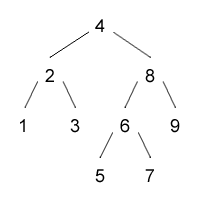
\includegraphics[width=.3\linewidth]{btree}
\caption{Binary tree}
\label{btree}
\end{figure}

We can now define various functions, for example to calculate the number of leafs (nodes without children) in the tree, or a function to test whether a value is a member of the binary tree. It is possible to use the data types in patterns, for example the \code{numLeafs} method first matches on an empty node, then a leaf node and finally on any other kind of node. The \code{isMember} method shows that the matching is not limited to one function parameter; the value to search for is taken as the first parameter and the binary tree as the second parameter.
\begin{verbatim}
  var numLeafs = fun(
    [Void, function() 0],              // empty node
    [Bt(_, Void, Void), function() 1], // leaf node
    [Bt(_, $, $), function(L, R) numLeafs(L) + numLeafs(R)]
  );

  var isMember = fun(
    [_, Void, function() false],
    [$, Bt($, $, $), function(x, v, L, R) x === v || 
      (isMember(x, L) || isMember(x, R))
    ]
  );

  numLeafs(bt);     // 5
  isMember(10, bt); // false
  isMember(3, bt);  // true
\end{verbatim}
The following two functions return a list of all the elements using in order and pre order traversals of the binary tree.
\begin{verbatim}
  var inorder = fun(
    [Void, function() []],
    [Bt($, $, $), function(v, L, R) inorder(L).concat([v], inorder(R))]
  );

  var preorder = fun(
   [Void, function() []],
   [Bt($, $, $), function(v, L, R) [v].concat(preorder(L), preorder(R))]
  );

  inorder(bt);      // [1,2,3,4,5,6,7,8,9]
  preorder(bt);     // [4,2,1,3,8,6,5,7,9]
\end{verbatim}
A real implementation of a binary tree would of course not use the data types and functions defined in this article for performance reasons, but a binary tree serves as a good introduction to both pattern matching and algebraic data types in JavaScript.

\section{Layout}
The layout module provides layout algorithms for laying out components. A component is an abstraction; it can be implemented in many ways, for example as items in a HTML5 Canvas drawing or as HTML elements. The module currently provides three layout algorithms: border, which lays out components in five different regions; grid, which lays out components in a user defined grid, and flex-grid which offers a grid with flexible column and row sizes.

The design of the layout module is inspired by the Java Swing layout managers \cite{sun08} and my own OpenGL based User Interface library \cite{stein06}. The module itself is not part of the core charting library but distributed as a separate library \cite{stein08} and bundled with a jQuery plugin for laying out HTML elements.

We start with the definition of a component; a component is something that has a minimum size, a preferred size, and a maximum size. It also has a method to set its size and position. A container is a component that contains other components and lays them out according to a layout algorithm (which are provided in the layout module.) Components need to satisfy the following interface requirements in order to be used with the layout algorithms; the component should have a:
\begin{itemize}
\item \code{bounds} property which returns the location and dimensions of the component;
\item \code{preferredSize}, \code{maximumSize}, and \code{minimumSize} properties which return the preferred, minimum and maximum size of the component respectively;
\item \code{insets} property which returns the offset between a container and its contents;
\item \code{isVisible} method which returns true if the component is visible;
\item \code{doLayout} method which might call a nested layout manager.
\end{itemize}

Note that the distinction between containers and components is artificial, both implement the same interface. 

\subsection{Border layout}
The border algorithm lays out components in five different regions. These regions are called center, north, south, east and west. The center component will be laid out in the center of the container, north on top of it, south beneath it and west and east on the left and right side respectively. The layout can only contain one of each region, but all are optional. Figure \ref{border} shows a visualization of a layout using all five regions. 

\begin{figure}[h!]
\centering
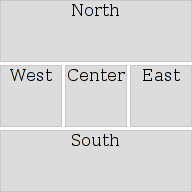
\includegraphics[width=.3\linewidth]{border}
\caption{Border layout with all five components present}
\label{border}
\end{figure}

The following example lays out a west, center and north component with a vertical space of 5 units between each component. There may be additional space between the components and the container if the container returns non-zero insets.
\begin{verbatim}
  var borderLayout = jLayout.border({
    west:   myWestComponent,
    center: myCenterComponent,
    north:  myNorthComponent,
    vgap: 5
  });

  borderLayout.layout(myContainer);
\end{verbatim}
If a region is not specified or the component is not visible its space will be taken up by the other components. 

\subsection{Grid layout}
The grid algorithms lays out the components in a grid, and resizes each component to the same size. The number of columns and rows can be specified by the user. Figure \ref{grid} shows a visualization of a grid layout with four components in a 2x2 grid. 

The following example lays out four components in a 2x2 grid, without any spacing between the components.
\begin{verbatim}
  var gridLayout = jLayout.grid({
    rows: 2,
    columns: 2,
    items: [myComponent1, myComponent2, myComponent3, myComponent4]
  });

  gridLayout.layout(myContainer);
\end{verbatim}

\begin{figure}[h]
\centering
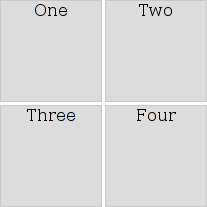
\includegraphics[width=.3\linewidth]{grid}
\caption{Grid layout with four components}
\label{grid}
\end{figure}

If the number of rows is given, the number of columns is calculated automatically by taking the number of components into account. If the number of rows is not given (or set to zero), and the number of columns is given, the number of rows will be automatically calculated using the number of components. If neither is given, the number of rows is set equal to the number of components and the number of rows is set to zero.

\subsection{Flex grid layout}
The flex grid algorithms lays out the components in a grid with flexible row and columns sizes. The number of columns and rows can be specified by the user. Figure \ref{flex-grid} shows a visualization of a flex grid layout with six components in a 3x2 grid. 

\begin{figure}[h]
\centering
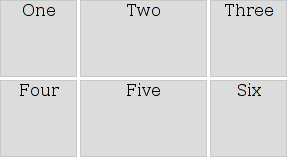
\includegraphics[width=.4\linewidth]{flexgrid}
\caption{Flex grid layout with six components}
\label{flex-grid}
\end{figure}

The interface to the flex grid is identical to that of the grid layout, and thus not further explained.

\section{Axis}
The axis module is a factory method for creating an object representation of a chart axis. The resulting object can represent two different kinds of axes: a numeric axis or a categoric axis. Axis themselves are not components that can be used by a layout manager. Instead they are parameters to the canvas module, which draws them (and is a component that can be laid out.) 

To create a numeric axis, the user supplies the axis module with an interval indicating the range the axis should span. The user can also optionally supply either an array of minor and major tick mark locations, or the desired number of minor and major tick marks.  When a number is supplied the axis module automatically calculates the tick locations in a visually pleasing manor, implemented using an algorithm described in the "Graphics Programming Gems" series \cite{heckbert90}. 

The algorithm boils down to choosing tick mark locations that have "nice" round numbers starting with either 1, 2, or 5. The algorithm favours these numbers over others. If such numbers are not desired, the user could always supply the axis module with custom values instead of having them automatically calculated based on the interval.

A categoric axis can be created by supplying the axis module with an array of labels. The axis module will then create an axis with an empty interval and use the supplied categories as labels.

All axes can also have a custom set of labels for the tick marks, and a label for the axis itself.

\section{Title}
The title module creates a title component, which simply draws a title and subtitle string on the screen. Both values are optional. No title or subtitle will be drawn if they are not supplied. Font information is retrieved from the default settings.

\section{Legend}
The legend module creates a component capable of drawing legend items.

It supports the following types of legend items: point (circle, cross, triangle, diamond, and square), line or bar. These three types are sufficient to represent all chart types currently supported in the library.

The legend component maintains a flow layout internally to lay out the individual legend items. This means the the items in a legend are dynamically arranged. If the legend is placed in a vertical position, the items will be laid out in one column, or given enough space multiple columns. When the legend is placed in a horizontal position, for example on top of a chart, the legend items will naturally "flow" into a row formation.

\section{Canvas}
The canvas module is responsible for setting up view-ports and drawing axes, labels and an optional grid. It supports three different types of axes: Cartesian, polar and categorical (which is a special instance of a Cartesian axis). Depending on the axes and drawing options given to it, it sets up a correct view-port and draws axes, tick marks, labels and the grid. 

The canvas module accepts an options object which should at least contain two Cartesian axes, or a polar axes. It might optionally also accept a hint for the aspect ratio of the canvas, and various boolean settings for turning on or off the drawing of---for example---axis lines, tick marks, labels, etcetera. Although all drawing options can be changed by the user, the defaults are chosen sensibly so as to cover most of the use cases. This results in the  default visual output for cartesian axes shown in Figure \ref{cartesianaxes}.

\begin{figure}[h!]
  \centering
  \subfloat[Two numeric axes]{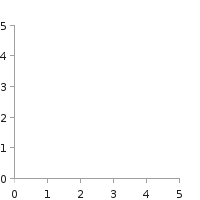
\includegraphics[width=0.3\textwidth]{numeric}}   
  \hspace{10pt}
  \subfloat[Numeric and categoric axis]{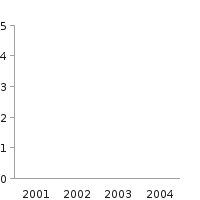
\includegraphics[width=0.3\textwidth]{numericcategoric}}
  \hspace{10pt}
  \subfloat[Two categoric axes]{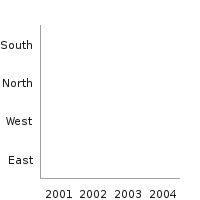
\includegraphics[width=0.3\textwidth]{categoriccategoric}}
  \caption{Different cartesian axis configurations}
  \label{cartesianaxes}
\end{figure}

A single polar axis determines the radius of the polar coordinate system. The axis is drawn in the horizontal position and duplicated in the vertical position. A visual representation is shown in Figure \ref{polar}.

\begin{figure}[h!]
\centering
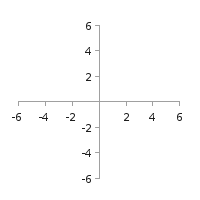
\includegraphics[width=.3\linewidth]{polar}
\caption{Polar coordinate system}
\label{polar}
\end{figure}

Both coordinate system do not draw a grid by default. Figure \ref{gridon} shows how grid lines are drawn when they are explicitly turned on. Note that the user can also choose to only draw the horizontal or vertical grid lines.

\begin{figure}[h!]
	\centering
	\subfloat[Cartesian grid]{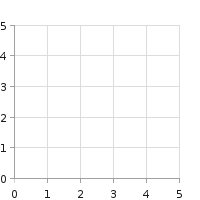
\includegraphics[width=0.3\textwidth]{numericgrid}}
	\subfloat[Polar grid]{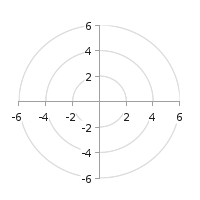
\includegraphics[width=0.3\textwidth]{polargrid}}
	\caption{Grid for cartesian and polar coordinate systems}
	\label{gridon}
\end{figure}

As the canvas is a component, it has a minimum and a preferred size. The minimum size of the canvas is calculated by the width and height of the labels of its major tick marks, plus some additional spacing between the labels. A canvas' preferred size is the size it would like to have to optimally display data. This includes the minimum size multiplied by the preferred aspect ratio. A canvas' maximum size is a user defined setting of the maximum width and height the chart may attain. By default, a chart will try to use exactly the space given to it by its drawing area unless it violates either the minimum or maximum size. In which case the drawing area will be resized.

The aspect ratio defines the dimensions of a chart. The ratio itself is defined by the horizontal and vertical axis or set by the user. If no ratio is given the library calculates it according to several heuristics aiming to reach an optimal $1:1$ ratio for most charts (other charts might have the golden ratio \cite{weisstein09, few04} set as default optimal value.) In order of importance, the heuristics are: 
\begin{itemize}
\item the resolution of the data (i.e. a maximum of one data point per screen pixel)
\item number and width of the axis labels
\item available space
\end{itemize}
The total size of a canvas is divided into two areas: a data area surrounded by padding necessary to contain all the labels. Figure \ref{outline} shows the data area marked by a red outline and the surrounding area marked with a blue outline.
\begin{figure}[h!]
\centering
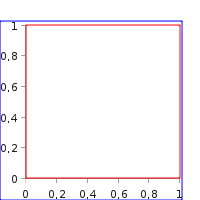
\includegraphics[width=.3\linewidth]{outline}
\caption{Data area and surrounding area outlines}
\label{outline}
\end{figure}

\section{Data}
The data module defines several data relationships and their corresponding input formats and validation routines. The chart plug-ins use these relationship definitions to declare the input they accept. Because not every data relationship can be predefined the data module is made extensible so that custom relationships can be constructed while still using some of the built in functionality.

A chart plug-in is not limited to accepting a single data relationship, it can declare an array of data relationships. The following list shows the definitions the available data relationships \cite{few06}:

\begin{description}
\item[Nominal comparison] To compare quantitative values for one or more categories.
\item[Time series] To display a relationship between quantitative values belonging to one or more categories and subdivisions of time.
\item[Distribution] To display the distribution of quantitative values over a range.
\item[Correlation] To display the correlation between a set of quantitative values.
\item[Function] To display an equation visually.
\end{description}

The three relationships which are not mentioned are: part to whole, ranking, and deviation. They have no explicit relationship type as they can be defined in terms of the other relationships. For example, deviation is a nominal comparison to a baseline, ranking is an ordered nominal comparison (ordinal), and part to whole is a nominal comparison with sub categories.

The data module accepts a single data object which contains both the data and meta-data. The meta-data properties consists of \code{categories} and \code{subcategories}, which are both optional. The overall structure of the data object is as follows:
\begin{alltt}
  var data = \{
    categories: [\ldots],
    subcategories: [\ldots],
    data: [\ldots]
  \};
\end{alltt}

All of the properties must be arrays. Both \code{category} and \code{subcategory} must not contain nested arrays. Sub-categories are the same for each category, which is enforced by the design of the data object. Although categories and sub-categories are nominal---and thus have no order---arrays are used because it is often desired to order them in a user defined way. The data format has no intrinsic time series type either, but because categories are ordered they can be used for that purpose. The data property can contain nested arrays, depending on if, and how, the \code{categories} and \code{subcategories} properties are used.
\begin{verbatim}
  var data = {
    categories: ['West', 'East'],
    data: [10, 12]
  };
\end{verbatim}

When \code{subcategories} is specified the data looks as follows, to---for example---define a time series with categories:
\begin{verbatim}
  var data = {
    categories: ['2001', '2002'],
    subcategories: ['West', 'East'],
    data: [
      [131, 120],
      [119, 141]
    ]
  };
\end{verbatim}

When none of the above rules meet the data, nested arrays are treated as multiple variables. For example, when the following data is given to chart that supports multiple variables it will be treated as $x, y$ coordinates in a single category.

\begin{verbatim}
  var data = {
    data: [
        [12, 4],
        [3, 11],
        [11, 2]
    ]
  };
\end{verbatim}

Normal JavaScript functions can be used to plot functions:

\begin{verbatim}
  function sine(x) {
    return Interval.sin(x);
  }
\end{verbatim}

The function is called using an interval and must also return an interval. Function plotting is explained in more detail in Chapter 3.5.

\section{Graphics}
The graphics module is an abstract layer built on top of the HTML5 Canvas API. It abstracts away less used methods and implements higher level functionality such the ability to create view-ports and to draw points in various ways.

The API is built on the chaining principle; methods return the object on which they were invoked. This allows for very succinct way of drawing graphics:
\begin{verbatim}
  graphics.
    beginPath().
      moveTo(10, 10).
	  lineTo(20, 20).
    endPath().
    stroke('#00000');
\end{verbatim}
The graphics API has two basic types of methods, one to create shapes and the other to create paths. Shapes include the following methods: \code{beginViewport}, \code{closeViewport}, \code{beginPath}, \code{stroke}, \code{fill}, \code{rect}, \code{line}, points (i.e. \code{circle}, \code{triangle}, \code{cross}, \code{diamond}, etc.), and \code{text}. Paths include the following methods: \code{lineTo}, \code{moveTo}, \code{arcTo}, \code{bezierCurveTo}, \code{quadraticCurveTo}, \code{closePath}, and \code{endPath}. Shapes can be considered ready-made instances of paths (although the implementation might differ) and they define a higher level interface to drawing complex paths.

The graphics object does not expose path methods, instead the \code{beginPath} method returns a set of functions that can create paths. Once the user is creating a path there is no way---other than by calling either the \code{closePath} or \code{endPath} methods (which returns the shapes set of methods)---to return to the shape group. This enforces the correct creation of paths and shapes (i.e. the API ensures that only valid method call combinations are made.)

\subsection{Custom view-ports}
The chart library implements its own transformation stack instead of using the one provided by the HTML5 Canvas API. The reason for this is to have complete control over how lines are drawn. This can only be achieved by not using the built-in transformation stack. An example of one of the problems is that line width is not implemented consistently across browsers and transformation states. Some browsers will use the line width associated with the transformation matrix when the path was created, while others will use the line width associated with the transformation matrix when the path was stroked. The following HTML5 Canvas example demonstrates this problem.
\begin{verbatim}
  ctx.lineWidth = 2;
  ctx.save();
  ctx.scale(1.5, 1.5);
  ctx.lineTo(10, 10);
  ctx.store();
  ctx.stroke();
\end{verbatim}
Some implementations will stroke the path with a line width of 2, while others will use a line width of 3 (2 scaled by 1.5). Unfortunately---and unlike other graphics APIs, such as OpenGL \cite{shreiner05}---the HTML5 Canvas element does not specify a stack for rendering properties such as line width. To overcome this problem, it was necessary to implement a custom transformation stack. The graphics module supports this through two methods: \code{beginViewport} and \code{closeViewport}. Instead of offering more general \code{scale} and \code{translate} methods, these methods deal with the concept of a viewport; a two dimensional area, with its own custom coordinate system. The \code{beginViewport} method takes four required parameters (\code{x}, \code{y}, \code{width}, and \code{height}) and three optional ones (horizontal interval, vertical interval, and polar.) When the horizontal and vertical intervals are specified, all drawing between the \code{beginViewport} and \code{closeViewport} method calls are performed in those intervals. This simplifies drawing data points by removing the need for transforming the data into the charts' view port; data can simply be plotted to the screen without transformation. Viewports can also be nested without problems.

The last optional parameter is polar, which, when turned on, transforms the coordinates to all drawing methods from polar to Cartesian. This makes it possible to also transparently plot polar data.

\subsection{Crisp line drawing}
Although it has support for some vector operations, the HTML5 Canvas element is not a vector based API, it basically draws bitmaps. As such, it becomes a necessity to manually ensure that lines are drawn on screen pixels instead of on pixel boundaries resulting in an approximation\cite{shepherd08} (blurred lines.) Figure \ref{crisp} shows two lines on a pixel grid. The red lines indicate the vector representation of the lines, and the blue filled area the actual screen pixels. The first line is drawn on pixel boundaries and thus results in an approximation, the right line on the other hand is drawn at exactly the center of a pixel and thus results in a crisp line drawing.

\begin{figure}[h!]
\centering
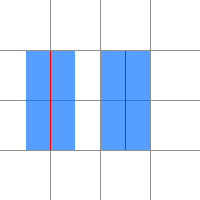
\includegraphics[width=.35\linewidth]{crisp}
\caption{Approximated line and crisp drawn line}
\label{crisp}
\end{figure}

The graphics module internally ensures that all lines and rectangles are drawn on screen pixels and never on the boundaries. As this "rounding" to screen pixels is done consistently, the resulting image is not affected, other than being slightly moved up or down (depending on the implementation of the rounding.)

\subsection{Fonts/Text support}
Unfortunately font and text drawing support in the HTML5 Canvas element is not well developed at the moment. Only Firefox 3.1 and Safari implement a standardized text drawing API. Firefox also offers its own alternative text drawing API. Both Internet Explorer and Opera have no support for drawing text on a HTML5 Canvas (Internet Explorer does in fact not support the Canvas element at all.) The standardized text API is also severely lacking in functionality. For example, it is possible to retrieve the width of a string in pixels, but not the height. Text is not treated as a set of paths, but drawn directly on the canvas through two separate \code{fillText} and \code{strokeText} functions. Strangely enough, the alternative Firefox text API does offer support for treating text as paths, and offers the ability to then stroke or fill those paths. Direct drawing versus paths is a not a big issue in the development of this chart library, but the font metrics problems are a big issue when aligning labels, legends, and titles.

In order to overcome these problems the chart library uses the HTML DOM to insert the a properly stylized string into an offscreen location in the surrounding HTML page and retrieve correct font metrics that way. In future versions of the library it might be possible to replace this with a better standardized and implemented HTML5 Canvas text API. Alternatively, it would be possible to overlay absolutely positioned HTML elements on top of the HTML canvas \cite{steele06}, use a bitmap font, or use one of the available path based fonts \cite{studt07, effenberger08, greenpoint08}.

\subsection{Browser support}
Firefox, Opera and Safari all support various subsets of the HTML5 Canvas tag. Fortunately there is a common subset of functionality that is sufficient for use in the chart library (apart from a text API.) Unfortunately, the only browser that does not support HTML5 Canvas is also the browser with the largest market share: Internet Explorer. Fortunately there are JavaScript implementations available that provide a HTML5 Canvas API for Internet Explorer and convert the API calls into VML elements \cite{google08}. By using one of these JavaScript implementations, the chart library supports all major browsers.

\section{Chart}
Each chart plug-in is an instance of the chart super \emph{class}\footnote{The word \emph{class} here does not imply classical inheritance, but rather a module that shares the same methods and some state with another module.}. The chart module takes care of the repetitive tasks, such as maintaining a layout, validating data, setting up a graphics context, parsing user options and so forth. Chart plug-ins can "inherit" from the chart module in the following way:

\begin{verbatim}
  Object.extend(defaults.type, {
     myChart: function (canvasIdentifier, data, options) {
       var that = {},
           my = {};
   
       that = chart(canvasIdentifier, options, my);
       
       Object.extend(that, {
         plot: function (g) {
           // draw the chart
         }
       });
       return that;
     }
  });
\end{verbatim}

This example first extends the \code{defaults.type} object discussed in the last section with a new chart type called \code{myChart}. It then creates two empty objects, one for the chart plug-in itself and one for any shared private (protected in classical inheritance) called \code{my}. The \code{that} object is then initialized using the chart constructor. The chart constructor parses the options and returns a chart component. The code then continues by overriding the plot function, which is called internally by the chart when it is drawn. When the plot function is called, the chart has already set up a view-port and drawn the axes and labels. This makes it especially easy to create new chart plug-ins. Plug-in authors can "inherit" from the chart module, perform any custom data parsing or validation and draw their chart in the plot function.

\section{Defaults}
The defaults "module" is not really a module, but a public object containing the default settings used in rendering charts. This includes colours, fonts, spacing between labels, point types and a list of all the available chart types. Users of the library can override any value in this object to suit their own needs.

The default colours come in two varieties: qualitative and diverging\cite{few08}. The qualitative set is used for displaying sub categories, to separate the items into distinct groups. The diverging set is used for encoding ranges, for example low to high. Both varieties have three subsets, one for highlighting values with strong hues and one for non-highlighted data with medium intensity hues. The last subset is a gray-scale version for printing. The hues themselves are taken from Cynthia Brewer's ColorBrewer application\footnote{\url{http://www.ColorBrewer.org} by Cynthia A. Brewer, Geography, Pennsylvania State University.}, which features many qualitative, sequential and diverging color palettes.

Other colours are kept muted [TODO: reference to Few \& Tufte?] so as to not distract from the data itself. Fonts default to simple black text, 11px in size and sans serif.





